 \documentclass[a4paper,twosided, 15pt]{book}
%\usepackage[czech]{babel} 
\usepackage[utf8]{inputenc}
\usepackage{listings}
\usepackage[T1]{fontenc}
\usepackage{float}
\usepackage{graphicx}
\usepackage{fancyhdr}
\usepackage{longtable}
\usepackage[usenames,dvipsnames]{color}
\usepackage{pifont}
\usepackage{wrapfig}
\usepackage[footnotesize,bf]{caption}
\usepackage[pdftex,colorlinks=true,linkcolor=blue,urlcolor=blue,pdftitle=MDS manual,pdfsubject=yyy,pdfkeywords=zzz,pdfauthor=Martin Madron,bookmarksopen=false,pdfpagemode=None]{hyperref}
\setcounter{chapter}{0} 
%\setcounter{chapter}{-1} 
\floatstyle{ruled}
\newfloat{code}{thp}{lop}
\floatname{code}{Code}

\definecolor{highlight_constant}{rgb}{0.333, 0.666, 0.0}
\definecolor{highlight_unknown_base}{rgb}{0.533, 0.133, 0.133}
\definecolor{highlight_comment}{rgb}{0.533, 0.533, 0.533}
\definecolor{highlight_symbol}{rgb}{0.666, 0.0, 1.0}
\definecolor{highlight_oper_sep}{rgb}{0.866, 0.533, 0.0}
\definecolor{highlight_directive}{rgb}{0.533, 0.533, 1.0}
\definecolor{highlight_label}{rgb}{0.533, 0.333, 0.0}
\definecolor{highlight_instruction}{rgb}{0.0, 0.0, 1.0}
\definecolor{highlight_sfr}{rgb}{0.0, 0.0, 0.866}
\definecolor{highlight_indirect}{rgb}{0.866, 0.0, 0.0}
\definecolor{highlight_imm_hex}{rgb}{0.666, 0.0, 0.866}
\definecolor{highlight_macro}{rgb}{0.8, 0.0, 0.866}
\definecolor{highlight_imm_dec}{rgb}{0.0, 0.533, 0.866}
\definecolor{highlight_hex}{rgb}{0.533, 0.0, 0.733}
\definecolor{highlight_oct}{rgb}{0.533, 0.0, 0.0}
\definecolor{highlight_dec}{rgb}{0.0, 0.333, 0.666}
\definecolor{highlight_bin}{rgb}{0.2, 0.2, 0.333}
\definecolor{highlight_string}{rgb}{0.533, 0.533, 0.0}
\definecolor{highlight_control}{rgb}{1.0, 0.0, 0.0}
\definecolor{highlight_imm_oct}{rgb}{0.666, 0.0, 0.0}
\definecolor{highlight_imm_bin}{rgb}{0.333, 0.333, 0.666}
\definecolor{highlight_char}{rgb}{0.0, 1.0, 1.0}
\definecolor{highlight_imm_constant}{rgb}{0.937, 0.737, 0.168}
\definecolor{highlight_imm_unknown}{rgb}{0.666, 0.2, 0.2}
\definecolor{highlight_lst_number}{rgb}{0.0, 0.882, 1.0}
\definecolor{highlight_lst_code}{rgb}{1.0, 0.2, 0.968}
\definecolor{highlight_lst_address}{rgb}{0.349, 0.356, 1.0}
\definecolor{highlight_lst_line}{rgb}{0.074, 0.003, 0.513}
\definecolor{highlight_lst_macro}{rgb}{0.533, 0.533, 0.533}
\definecolor{highlight_lst_include}{rgb}{0.533, 0.533, 0.533}
\definecolor{highlight_lst_msg}{rgb}{0.0, 0.0, 0.0}
\newcommand{\menuitem}[1]{\texttt{#1}}
\newcommand{\fileextension}[1]{\texttt{#1}}
\newcommand{\mysmallfont}{\fontsize{8pt}{10pt} \selectfont{}}
\newcommand{\uC}{$\mu$C }

\pdfadjustspacing=1
\raggedbottom

\pagestyle{fancy}
\fancyhf{}
\fancyhead[EL,OR]{\bfseries\thepage}
\fancyhead[LO]{\bfseries\rightmark}
\fancyhead[RE]{\bfseries\leftmark}

\fancypagestyle{plain}{
	\fancyhead{}
	\fancyhead[EL,OR]{\bfseries\thepage}
	\renewcommand{\headrulewidth}{0pt}
}


%%%%%%%%%%%%%%%%%%%%%%%%%%%%%%%%%%%%%%%%%%%%%%%%
 %%%%%%%%%%%%%%%%%%%%%%%%%%%%%%%%%%%%%%%%%%%%%%%%%%%%%%%
\title{Multiplatform Development Environment \\
2013/2014}
\author{Moravia Microsystems s.r.o \\}

%%%%%%%%%%%%%%%%%%%%%%%%%%%%%%%%%%%%%
\begin{document}
\maketitle
  
        \begin{center}
        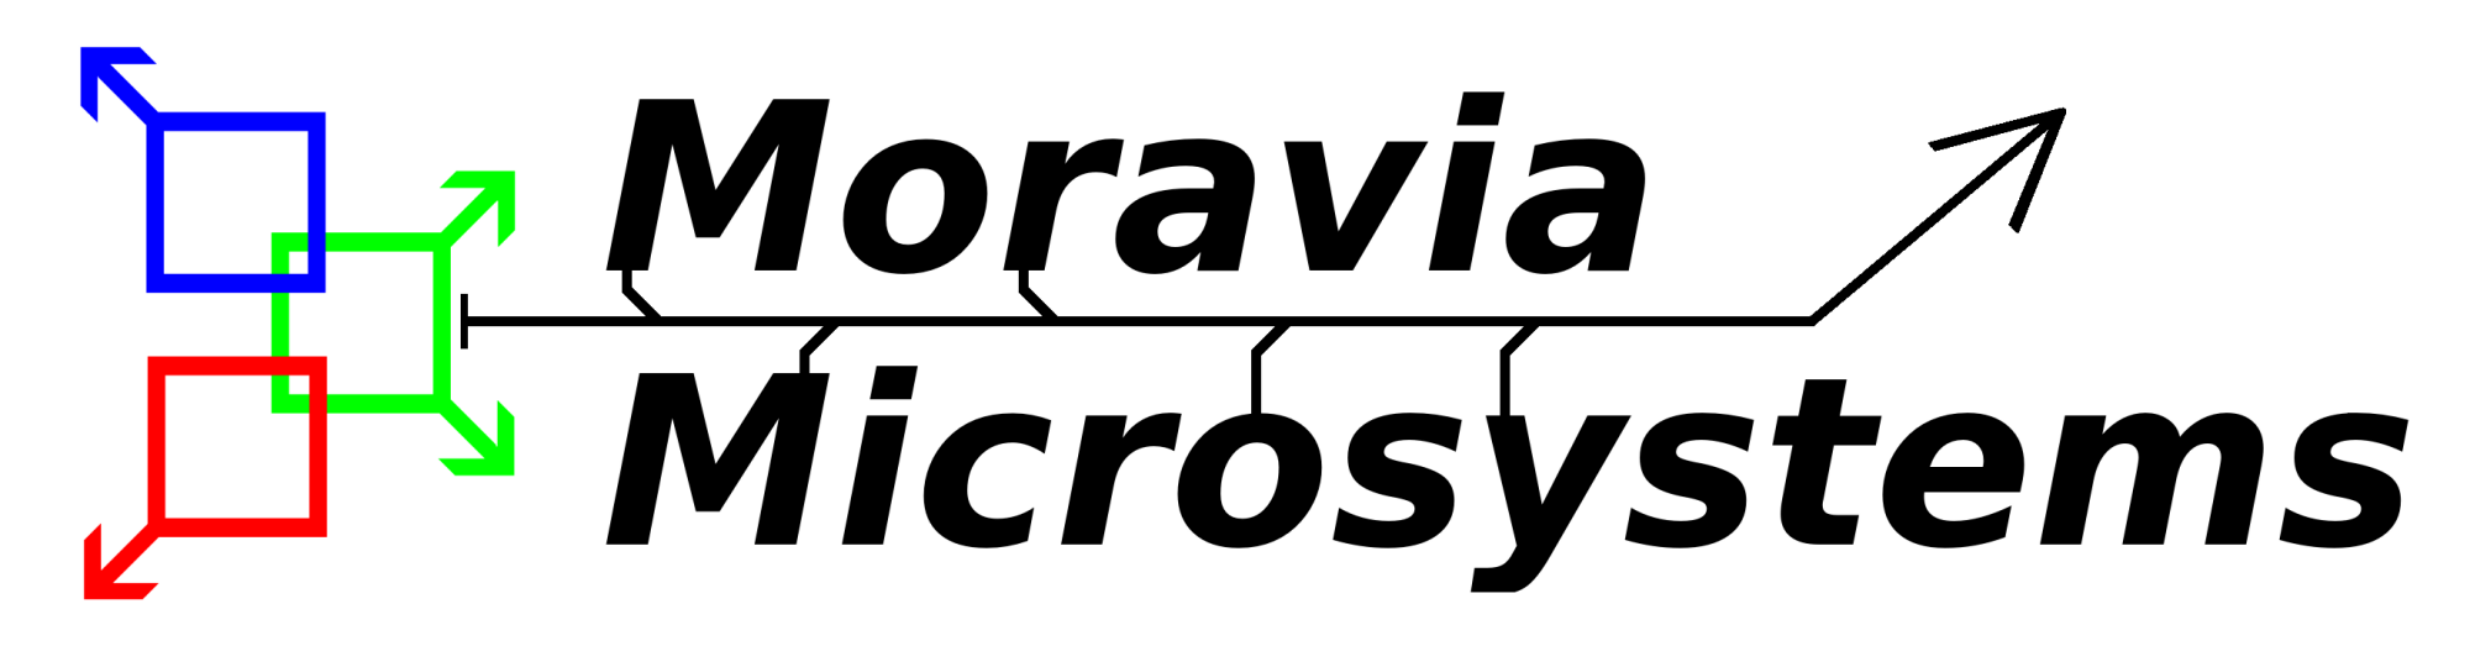
\includegraphics[scale=0.1]{./Moravia_Microsystems.png}
        \end{center}


\newpage
\tableofcontents
\newpage

\chapter{Preface}
This manual is an introduction to the Moravia Microsystems development tools designed for microcontrollers.
It introduces the MDS Integrated Development Environment, Simulator and 
presents a step-by-step guided tour of the numerous features and capabilities 
the Moravia Microsystems embedded development tools offer.
  
\chapter{About MDS}
MDS is a window-based software development platform that 
combines a robust and modern editor with a project manager 
and make facility tool. It integrates all the tools needed
to develop embedded applications including a C/C++ compiler, macro
assembler, linker/locator, and a HEX file generator. MDS helps
expedite the development process of embedded applications by providing
the following: 
        \section{Features}
                \begin{itemize}
                    \item Full-featured source code editor
                    \item Project Manager for creating and maintaining your projects
                    \item Integrated Make Utility functionality for assembling, compiling, and linking your embedded applications
                    \item Test bench - Displays changes of values on a time graph. Study the signal and variable changes and view their dependency. Simulates all possible outside conditions
                \end{itemize}

	\section{Requirements}
	
\chapter{Quick start}
        \section{Demonstration project}
        The aim of the demonstration project is to provide an easy way to explore
        the IDE without reading long documents. The
        demonstration project can be opened from the welcome dialog ( Main Menu
        Help Welcome dialog Open demonstration project. )
        Demonstration project should introduce new user into usage of the most
        common functions of the IDE like assembling the code, running simulator
        and so on. Demonstration project cannot be modified by the user in order
        to make it less volatile.
                \begin{figure}
                    \centering{}
                    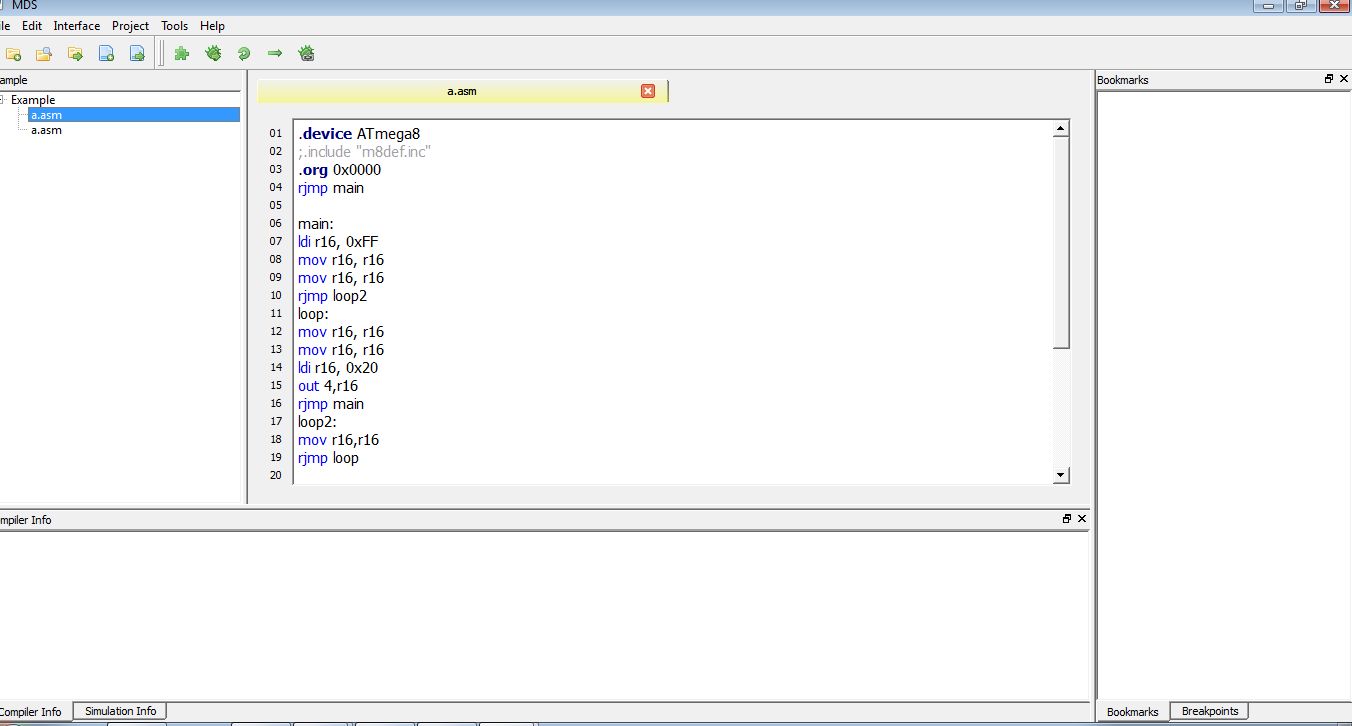
\includegraphics [scale=0.4]{img/Demonstration_project.png}
                    \caption{Demonstration project}
                \end{figure}
        \section{Your first project}
  
        \section{What is PicoBlaze?}
        PicoBlaze is the designation of a series of three free soft processor cores
        from Xilinx for use in their FPGA and CPLD products. They are based on a RISC
        architecture of 8 bits and can reach speeds up to 100 MIPS on the Virtex 4
        FPGA's family. The processors have an 8-bit address and data port for access
        to a wide range of peripherals. The license of the cores allows their free
        use, albeit only on Xilinx devices, and they come with development tools.
        All instructions execute in two clock cycles, making performance of the core instruction
        set deterministic. Interrupt response is not more than five clock cycles. As a resource
        optimization, it is possible for two PicoBlaze cores to share the same 1k x 18 instruction
        PROM, taking advantage of the dual-ported implementation of this block on Xilinx FPGAs.
        
                \subsection{PicoBlaze features:}
                        \begin{itemize}
                                \item 16 byte-wide general-purpose data registers
                                \item 1K instructions of programmable on-chip pr
                                        ogram store, automatically loaded during
                                        FPGA configuration
                                \item Byte-wide Arithmetic Logic Unit (ALU) with CARRY and ZERO indicator flags
                                \item 64-byte internal scratchpad RAM
                                \item 256 input and 256 output ports for easy expansion and enhancement
                                \item Automatic 31-location CALL/RETURN stack
                                \item Predictable performance, always two clock cy
                                        cles per instruction, up to 200 MHz or
                                        100 MIPS in a Virtex-II Pro FPGA
                                \item Fast interrupt response; worst-case 5 clock cycles
                                \item Optimized for Xilinx Spartan-3, Virtex-II, and Virtex-II Pro FPGA architectures just
                                        96 slices and 0.5 to 1 block RAM
                                \item Assembler, instruction-set simulator support
                        \end{itemize}

\chapter{User interface}        
         \section{Window Layout Concept}
          Developers can define their working environment to fit the needs and 
          preferences. For a better understanding of further comments and instructions,
          five major screen areas are defined. % pops�no v obr�zku
               \begin{figure}
                      \centering
                      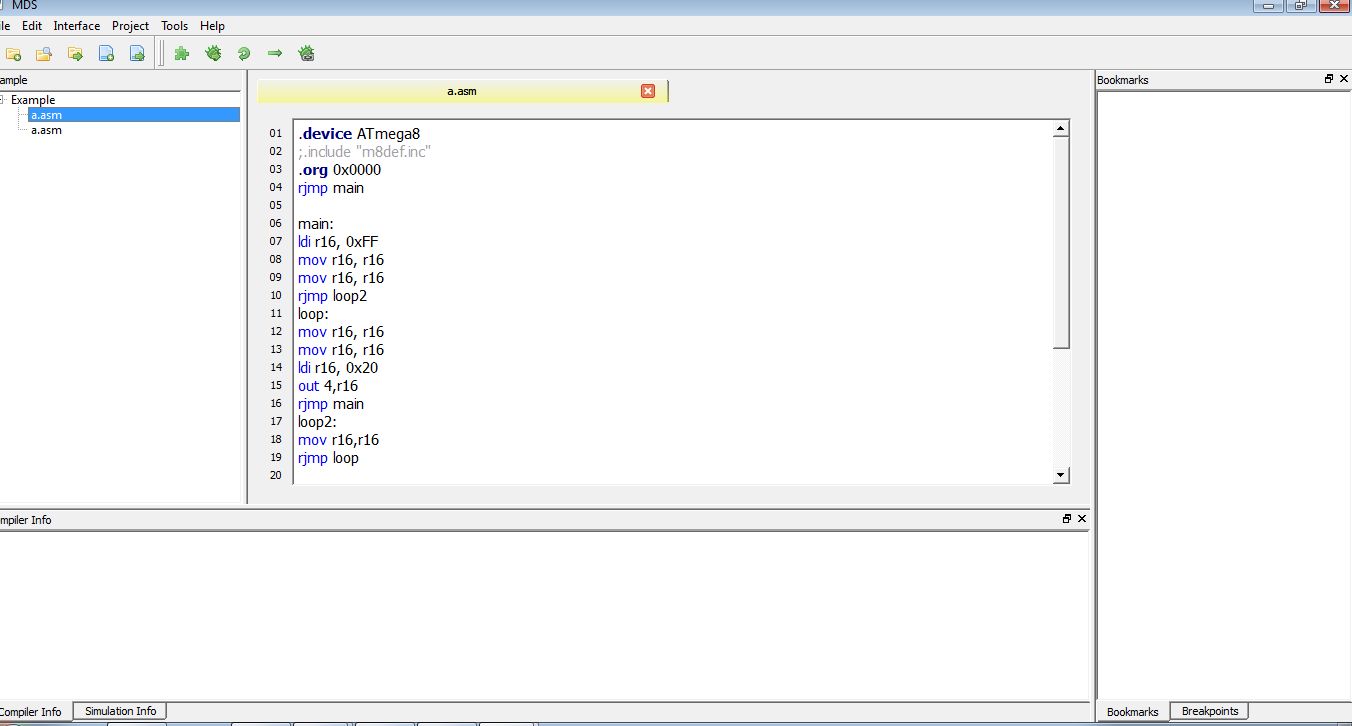
\includegraphics [scale=0.3]{img/Demonstration_project.png}
                      \caption{Window layout concept}
               \end{figure}
                         
                \subsection{Source code editor}
                \subsection{Top panel}
                        \begin{wrapfigure}{r}{0pt}
                                \centering
                                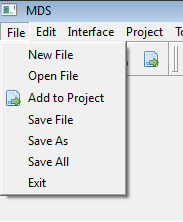
\includegraphics[width=110pt]{img/menu_file.png}
                                \caption{File selection}
                        \end{wrapfigure}
                        
                        \begin{itemize}
                            \item New file: creates a new document to enter a new source file.
                            \item Open file: allows to open an existing source file.
                            \item Open recent: lists the 5 most recently used files.
                            \item Add to project:
                            \item Save file: saves the open document to the related file.
                            \item Save as: save the open document to a new file.
                            \item Save all: saves all currently open documents.
                            \item Exit: closes all open documents and closes MDS.
                        \end{itemize}
                        
                        \begin{wrapfigure}{r}{0pt}
                                \centering
                                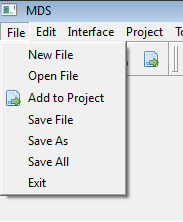
\includegraphics[width=110pt]{img/menu_file.png}
                                \caption{Edit selection}
                        \end{wrapfigure}
               
                        \begin{itemize}
                            \item Undo: will undo all edit actions on the open document in reverse order
                            \item Redo: will redo all undo actions
                            \item Cut: cuts all selected parts of the open doecument and puts it on the clipboard
                            \item Copy: copies all selected parts of the open document to the clipboard
                            \item Paste: pastes the text contents of the clipboard in the open document
                            \item Select: All selects all text in the open document
                            \item Find: find a to be given string through the open document
                            \item Replace: replace a given string in the open document by a new string
                        \end{itemize}

                        \begin{wrapfigure}{r}{0pt}
                                \centering
                                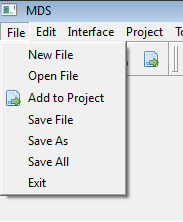
\includegraphics[width=110pt]{img/menu_file.png}
                                \caption{Project selection}
                        \end{wrapfigure}

                        \begin{itemize}
                            \item Undo: will undo all edit actions on the open document in reverse order
                            \item Redo: will redo all undo actions
                            \item Cut: cuts all selected parts of the open doecument and puts it on the clipboard
                            \item Copy: copies all selected parts of the open document to the clipboard
                            \item Paste: pastes the text contents of the clipboard in the open document
                            \item Select: All selects all text in the open document
                            \item Find: find a to be given string through the open document
                            \item Replace: replace a given string in the open document by a new string
                        \end{itemize}
              
                \subsection{Bottom panel}
                \subsection{Right panel}
                \subsection{Left panel}
         \section{Other tools}        
        
                \subsection{Code Completion list}
                The Code Completion List shows program symbols that contain
                the characters you are currently typing.
                        \begin{figure}
                            \centering{}
                            
\includegraphics [scale=0.3]{img/mensi_obrazek.png}
                            \caption{Code completion list}
                        \end{figure}

                \subsection{Parameter Information}
                Parameter Information shows the names, amount of, and
                parameter types of a function or method. The parameter in bold
                indicates the next parameter that is required as you are typing.
                        \begin{figure}
                            \centering{}
                            
\includegraphics [scale=0.3]{img/mensi_obrazek.png}
                            \caption{Parametr information list}
                        \end{figure}

                \subsection{Syntax Checking}
                Syntax Checking validates the program syntax while you are typing
                the code and provides real-time alerts to potential code violations
                before compilation. This enhances productivity and greatly reduces
                edit, compile, and correction cycles.
                    \begin{figure}
                        \centering{}
                        
\includegraphics [scale=0.3]{img/mensi_obrazek.png}
                        \caption{Syntax checking picture}
                    \end{figure}

                \subsection{Instruction details}
                \subsection{Subprograms call monitor}
                \subsection{ASCII chart}
                \subsection{PicoBlaze Instruction Table}
                \subsection{Symbol viewer}
                \subsection{Stopwatch}

                \subsection{Hexadecimal editors }
                \subsection{Interrupt monitor}

                \subsection{Number base converter}
                This tool is very usefull, when you want to find out the representation of given number in other
                number bases.

                        \begin{wrapfigure}{r}{0pt}
                                \centering
                                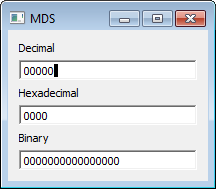
\includegraphics[width=110pt]{img/convertor.png}
                                \caption{Convertor}
                        \end{wrapfigure}

                \subsection{8-segment editor}
                With this tool you can easily determine what
                value you have to set on a port to display a digit
                on a numerical LED display. In the left part of
                the dialog window, you can find numerical val
                ues corresponding to the digit displayed in the
                middle part. These values are represented for
                both common cathode and anode and in three
                numerical bases, hexadecimal, decimal and oc
                tal. Buttons on left side from entry boxes copies
                value from adjacent entry box into clipboard.
                In the right part of the window you can set what port pin is connected to
                what LED segment.
                        \begin{wrapfigure}{r}{0pt}
                            \centering{}
                            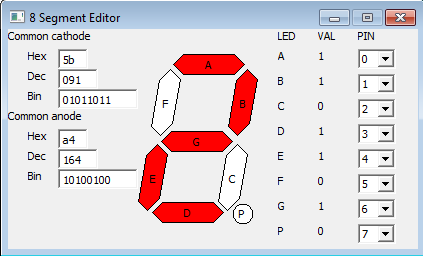
\includegraphics[width=110pt]{img/8segment.png}
                            \caption{8-segment editor}
                        \end{wrapfigure}


\chapter{MCU simulator}
  	\section{Short introduction}
        The MCU simulator is a tool designed to mimics behavior of a real MCU as
        much as possible. But it can have certain limitations, the most expectable
        limitation is of course the speed of simulation. This simulator is very slow,
        but ofers some extra features.
        \section{Modes of simulation}
        There are 4 modes of simulation:
            \begin{itemize}
                \item STEP: Execute exactly one intruction, no matter how many machine
                        cycles it will take. This does not apply for macro-instruction,
                        in that case each instruction of the macro is executed separately.
                \item STEP OVER: Execute as many instructions as possible until simulator
                cursor changes its location from one line of source code to another.
                \item ANIMATE: Do the same as step, but in a loop, one after another until
                stopped by a waring condition or user request.
                \item RUN: This is generally the same as animate, but much faster, because
                GUI is not updated so often as in the animate mode.
                \item STEP BACK: Take back the last performed step. There is limited number
                of step which can be taken back.
            \end{itemize}
            
\chapter{Built-in Macro assembler}
In this chapter, we will be concerned with MDS build-in assembler.
With syntax of its statements, directives and PicoBlaze assembler instructions.
It is assumed, that the reader is familiar with general concepts of assembly 
language programming and PicoBlaze architecture.

        \section{Predefined Symbols}
        There are symbols which are defined by default by assembler. The aim is to
        make it a little easier to write code in assembly language for 8051,
        because user don not have to define all these symbols in his or her code.
        This feature can be turned of by ``\texttt{\$NOMOD}'' control sequence.
		\begin{table}[h!]
			\centering{}
			\mysmallfont{}
			\caption{Code addresses}
			\begin{tabular}{|ll|ll|ll|ll|}
				\hline
				\textbf{Symbol}	& \textbf{Value}
					& \textbf{Symbol} & \textbf{Value}
					& \textbf{Symbol} & \textbf{Value}
					& \textbf{Symbol} & \textbf{Value} \\
				\hline
				RESET	& 000h	& EXTI0	& 003h	& TIMER0& 00Bh	& EXTI1	& 013h \\
				TIMER1	& 01Bh	& SINT	& 023h	& TIMER2& 02Bh	& CFINT	& 033h \\
				\hline
			\end{tabular}
		\end{table}
%%%%%%%%%%%%%%%%%%%%%%%%%%%%%%%%%%%%%%%%%%%%%%%%%%%%%%%%%%%%%%%%%%%%%%%%%%%
 	\section{Statements}
        Source code files for this assembler must be text files where lines are formed like these:\\
		\\ {
                \mysmallfont{}
                \texttt{}
                \begin{tabular}[h!]{llll}
                        \verb'[' { \color{highlight_label} label: } \verb']' &
                        \verb'[' { \color{highlight_instruction} instruction } &
                        \verb'[' { \color{highlight_symbol} operand } \verb'[' , { \color{highlight_symbol} operand } \verb'[' , { \color{highlight_symbol} operand } \verb']' \verb']' \verb']' &
                        \verb'[' { \color{highlight_comment} ;comment } \verb']' \\

                        \verb'[' { \color{highlight_label} label: } \verb']' &
                        { \color{highlight_directive} directive } &
                        \verb'[' { \color{highlight_symbol} argument } \verb']' &
                        \verb'[' { \color{highlight_comment} ;comment } \verb']' \\

                        { \color{highlight_constant} symbol } &
                        { \color{highlight_directive} directive } &
                        { \color{highlight_symbol} argument } &
                        \verb'[' { \color{highlight_comment} ;comment } \verb']' \\
                \end{tabular}
                    }
                \bigskip
        Everything in square brackets is optional. Compilation does not go be-
        yond line containing "end" directive, so after that directive the code do not
        have to be syntactically valid. Empty lines are allowed as well as line contain-
        ing only comment or label. Statements can be separated by spaces, NBSP
        characters and tabs. Statements are case insensitive and their length is not
        limited, overall line length is also not limited.

%%%%%%%%%%%%%%%%%%%%%%%%%%%%%%%%%%%%%%%%%%%%%%%%%%%%%%%%%%%%%%%%%%%%%%%%%%%%%% 
    	\section{Symbols}
        Symbol names for numbers, macros or addresses defined by user in the code using
        appropriate directive. Like with ``\texttt{equ}'' directive you can define a new
        symbol and assign a value to it right away. Symbols may consist of upper and lower
        case letter, digits and underscore character (``\_''), their length is not limited,
        they are case insensitive and they can be the same as language keywords. Be aware of
        that there cannot coexists two or more symbols in the same memory segment which differs
        only by letter casing, in other words symbols ``\texttt{abc}'' and ``\texttt{ABC}''
        are completely the same thing.
                \begin{code}[h!]
                        \mysmallfont{}
                        {\color{highlight_comment}\verb'; Example of symbol definition'}\\
                        {\color{highlight_constant}\verb'First_symb'}\verb'    '{\color{highlight_directive}\verb'EQU'}\verb' '{\color{highlight_bin}\verb'0b100111'}\verb'   '{\color{highlight_comment}\verb'; Number in binary'}\\
                        {\color{highlight_constant}\verb'Second_symb'}\verb'   '{\color{highlight_directive}\verb'SET'}\verb' '{\color{highlight_oct}\verb'47q'}\verb'       '{\color{highlight_comment}\verb'; Octal'}\\
                        {\color{highlight_constant}\verb'Third_symb'}\verb'    '{\color{highlight_directive}\verb'REG'}\verb' '{\color{highlight_dec}\verb'39d'}\verb'       '{\color{highlight_comment}\verb'; Decimal'}\\
                        {\color{highlight_constant}\verb'Fourth_symb'}\verb'   '{\color{highlight_directive}\verb'DATA'}\verb' '{\color{highlight_hex}\verb'27h'}\verb'       '{\color{highlight_comment}\verb'; Hexadecimal'}\\
                        {\color{highlight_constant}\verb'Fifth_symb'}\verb'    '{\color{highlight_directive}\verb'CODE'}\verb' '{\color{highlight_hex}\verb'27h'}\verb'       '{\color{highlight_comment}\verb'; Hexadecimal'}\\
                        % Caption
                        \caption{An example of symbol definitons}
                \end{code}
        As you can see in Code 1 example, some unknown directives are used for symbol definition. Next chapter describes all directives, as well
        as constants syntax and expresions priority.

	\section{Constants} 
        MDS supports both prefix and sufix definition. 
                \begin{code}[h!]
                    \mysmallfont{}
                            {\color{highlight_comment}\verb'; Example of constants syntax'}\\
                            {\color{highlight_constant}\verb'10'}\verb' '\verb'   '{\color{highlight_comment}\verb'; Decimal'}\\
                            {\color{highlight_constant}\verb'10D'}\verb' '\verb'   '{\color{highlight_comment}\verb'; Decimal'}\\
                            {\color{highlight_constant}\verb'0xFE'}\verb' '\verb'   '{\color{highlight_comment}\verb'; Hexadecimal'}\\
                            {\color{highlight_constant}\verb'FEh'}\verb' '\verb'   '{\color{highlight_comment}\verb'; Hexadecimal'}\\
                            {\color{highlight_constant}\verb'O52'}\verb' '\verb'   '{\color{highlight_comment}\verb'; Octal'}\\
                            {\color{highlight_constant}\verb'52q'}\verb' '\verb'   '{\color{highlight_comment}\verb'; Octal'}\\
                            {\color{highlight_constant}\verb'01011110b'}\verb' '\verb'   '{\color{highlight_comment}\verb'; Binary'}\\
                            {\color{highlight_constant}\verb'0b00100001'}\verb' '\verb'   '{\color{highlight_comment}\verb'; Binary'}\\
                            {\color{highlight_constant}\verb'0b01'}\verb' '\verb'   '{\color{highlight_comment}\verb'; Binary, considers left side of byte zeroes'}\\
                            {\color{highlight_constant}\verb'01b'}\verb' '\verb'   '{\color{highlight_comment}\verb'; Binary, considers right side of byte zeroes'}\\
            % 	        {\color{highlight_constant}\verb'\'s\''}\verb' '\verb'   '{\color{highlight_comment}\verb'; Character'}\\
            % 	        {\color{highlight_constant}\verb'\'\n\''}\verb' '\verb'   '{\color{highlight_comment}\verb'; Character'}\\
                                    % Caption
                    \caption{Constants syntax}
                \end{code}
    
                \subsection{Using constants in code}
                When you want to load constant directly to register, or use it as a label, you need to tell the compiler, that you are using
                constant. It is done bz adding "\#" before constant. See examples below.
                        \begin{code}[h!]
                            \mysmallfont{}
                            {\color{highlight_comment}\verb'; Example of direct constant load into register'}\\
                            {\color{highlight_constant}\verb'10'}\verb' '\verb'   '{\color{highlight_comment}\verb'; Decimal'}\\
                            {\color{highlight_constant}\verb'10D'}\verb' '\verb'   '{\color{highlight_comment}\verb'; Decimal'}\\
                            % Caption
                            \caption{Constants in code}
                            \end{code}
		
        \section{Expressions}
        Arithmetical expressions are evaluated at compilation time and replaced by assembler
        with constant corresponding the their resulting value. Expressions comprises of arithmetical operators,
        constants, symbols and another expressions. An example of such expression might be
                \begin{itemize}
                    \item  \texttt{2+1}
                    \item  \texttt{(2 + 4) - ABC}
                    \item  \texttt{A \&\& B)} (
                    \item  \texttt{X XOR 0FF00H}
                    \item  \texttt{X * Y + X \% Y}
                \end{itemize}
	
        When multiple operators occur in an expression, the expression is evaluated in a specific order depending upon the operators in the expression.
        All LOGICAL operators have priorities lower than
        arithmetic and relational operators. Therefore, if an expression involving arithmetic, relational and logical operators, the arithmetic
        operators are evaluated first, followed by the relational operators, followed by the logical operators.
        The following table shows the priority of all the operators used in expressions.
		\begin{table}[h!]
			\mysmallfont{}
			\centering{}
			\begin{tabular}{|l|l|l|}
				\hline
				Operator	& Description			& Example		\\\hline
				\multicolumn{3}{|l|}{\textbf{Unary Operators}} \\\hline
				NOT		& one's complement		& NOT 0a55ah		\\\hline
				HIGH		& high order byte		& HIGH 0a55ah		\\\hline
				LOW		& low order byte		& LOW 0a55ah		\\\hline
				\multicolumn{3}{|l|}{\textbf{Binary Operators}} \\\hline
				+		& unsigned addition		& 11 + 12		\\\hline
				-		& unsigned subtraction		& 13 + 11		\\\hline
				*		& unsigned multiplication	& 3 * 5			\\\hline
				/		& unsigned division		& 20 / 4		\\\hline
				MOD		& unsigned remainder		& 21 MOD 4		\\\hline
				SHL		& logical shift left		& 32 SHL 2		\\\hline
				SHR		& logical shift right		& 32 SHR 2		\\\hline
				AND		& logical and			& 48 AND 16		\\\hline
				OR		& logical or			& 370q OR 7		\\\hline
				XOR		& exclusive or			& 00fh XOR 005h		\\\hline
				.		& bit operator			& P1.4			\\\hline
				EQ, = 		& equal to			& 11 EQ 11		\\\hline
				NE, <>		& not equal to			& 11 NE 11		\\\hline
				LT, < 		& less than			& 11 LT 12		\\\hline
				LE, <=		& less or equal than		& 11 LT 11		\\\hline
				GT, > 		& greater than			& 12 GT 11		\\\hline
				GE, >=		& greater or equal than		& 12 GT 11		\\\hline
			\end{tabular}
			\caption{Expression operators}
		\end{table}
		
% 				{%
% 		\newcommand{\mc}[3]{\multicolumn{#1}{#2}{#3}}
% 		\begin{center}
% 		  \begin{longtable}[t]{llll}\hline
% 			  \mc{1}{|l|}{Priority} & \mc{1}{l|}{Name} & \mc{1}{l|}{Operator} & \mc{1}{l|}{Example}\\\hline
% 			  1		& 		Bitwise NOT		 & 		~ & 		~0xFF\\
% 			  � 		& Logical NOT & 		! &		 !A\\
% 			  2 		& nasobeni 		&		 * &		 A * B\\
% 			  � & deleni & / & A / B\\
% 			  � & modulo & % & A % B\\
% 			  3 & scitani & + & A + B\\
% 			  � & Odcitani & - & A - B\\
% 			  4 & Binary shift left & << & A << 4\\
% 			  � & Binary shift right & >> & A >> 4\\
% 			  5 & mensinez & < & A < B\\
% 			  � & vetsinez & > & A > B\\
% 			  � & mensineborovno & <= & A <= B\\
% 			  � & vetsineborovno & >= & A >= B\\
% 			  6 & Equal to & == & A == B\\
% 			  � & ruzneod & != & A != B\\
% 			  7 & Bitwise AND & & & A & B\\
% 			  8 & Bitwise OR & | & A | B\\
% 			  9 & Bitwise XOR & ^ & A ^ B\\
% 			  10 \& Logical AND & && & A && B\\
% 			  11 \& Logical OR & || & A || B
% 		  \end{longtable}
% 		\end{center}
% }%		
        A priority of 1 is the highest priority a priority of 7 is the lowest priority.
        When operators with different priority levels appear in an expression, operations are performed
        according to priorities. When operators of the same priority appear in an expression, operations are performed from left to right within
        the expression.

        \section{Assembler directives}
        Assembly directives are instructions
        that are executed by an assembler at assembly time,
        not by a CPU at run time. They can make the assembly of the program
        dependent on parameters input by a programmer, so that one program can be
        assembled different way, perhaps for different applications. They also
        can be used to manipulate presentation of a program to make it easier to read and maintain\\
        The specified format for most of the directives is:
		 \\	
                 \\ {
                \texttt{}
                \begin{tabular}[h!]{llll}
                { \color{highlight_symbol} <symbol> }  &
                    { \color{highlight_directive} <directive> } &
                    { \color{highlight_constant} <expresion> } & { \color{highlight_comment} ; Directive syntax }\\
                \end{tabular}
      		 }
                 \\
        This syntax is valid for directives EQU, SET, REG, DATA, CODE, DEFINE
        MDS also supports some special PicoBlaze directives, with diferent syntax format, which is  
         \\      {		
                \texttt{}
                \begin{tabular}[h!]{llll}
                        { \color{highlight_directive} <directive> } &
                        { \color{highlight_constant} <expresion> } & { \color{highlight_comment} ; Directive syntax }\\
                \end{tabular}
      		 } 
           \\
        Those directives are CONSTANT, VARIABLE, ADRESS and NAMEREG.
             
                \subsection{EQU}
                \textbf{SYNTAX:}\\
                        \\ {
                            \texttt{}
                            \begin{tabular}[h!]{llll}
                                    { \color{highlight_symbol} <symbol> }  &
                                    { \color{highlight_directive} EQU } &
                                    { \color{highlight_constant} <expresion> } & { \color{highlight_comment}  }\\
                            \end{tabular}
                        }\\
                        \\
                \textbf{DESCRIPTION:}\\
                The directive EQU stands for "equals"; it allows you to give a numerical value to a label.
                \\
                \textbf{EXAMPLE:}\\
                
                        \begin{code}[h!]
                        \mysmallfont{}
                                {\color{highlight_constant}\verb'First_symb'}\verb'    '{\color{highlight_directive}\verb'EQU'}\verb' '{\color{highlight_bin}\verb'0b10011100'}\verb'   '{\color{highlight_comment}\verb'; Number in binary'}\\
                                {\color{highlight_constant}\verb'Second_symb'}\verb'   '{\color{highlight_directive}\verb'EQU'}\verb' '{\color{highlight_oct}\verb'47'}\verb'       '{\color{highlight_comment}\verb'; Decimal'}\\
                                {\color{highlight_constant}\verb'Third_symb'}\verb'    '{\color{highlight_directive}\verb'EQU'}\verb' '{\color{highlight_dec}\verb'0x39'}\verb'       '{\color{highlight_comment}\verb'; Hexadecimal'}\\
                        \caption{Using EQU directive}
                    \end{code}

            In this example, the assembler would always replace {\color{highlight_symbol}\verb'First_symb'} with 0x9C,
            {\color{highlight_symbol}\verb'Second_symb'} with 0x2F and {\color{highlight_symbol}\verb'Third_symb'} with 0x39.

                \subsection{CONSTANT}
                \textbf{SYNTAX:}\\
                    \\ {
                        \texttt{}
                        \begin{tabular}[h!]{llll}
                                { \color{highlight_directive} CONSTANT } &
                                { \color{highlight_symbol} <symbol> }  &
                                \verb',' &
                                { \color{highlight_constant} <expresion> }\\
                        \end{tabular}
                    }\\
                    \\
                \textbf{DESCRIPTION:}\\
                The directive CONSTANT allows you to give a numerical value to a label. It is same like EQU, but with diferent syntax.\\

                \textbf{EXAMPLE:}\\
                    \begin{code}[h!]
                        %\mysmallfont{}
                                {\color{highlight_directive}\verb'CONSTANT'}\verb'    '{\color{highlight_symbol}\verb'First_symb'}\verb','{\color{highlight_constant}\verb'0b10011100'}\verb'   '{\color{highlight_comment}\verb'; Number in binary'}\\
                                {\color{highlight_directive}\verb'CONSTANT'}\verb'    '{\color{highlight_symbol}\verb'Second_symb'}\verb','{\color{highlight_constant}\verb'47'}\verb'       '{\color{highlight_comment}\verb'; Decimal'}\\
                                {\color{highlight_directive}\verb'CONSTANT'}\verb'    '{\color{highlight_symbol}\verb'Third_symb'}\verb','{\color{highlight_constant}\verb'0x39'}\verb'       '{\color{highlight_comment}\verb'; Hexadecimal'}\\
                        \caption{Using CONSTANT directive}
                    \end{code}

                In this example, the assembler would always replace {\color{highlight_symbol}\verb'First_symb'} with 0x9C,
                {\color{highlight_symbol}\verb'Second_symb'} with 0x2F and {\color{highlight_symbol}\verb'Third_symb'} with 0x39.

            \subsection{SET}
            \textbf{SYNTAX:}\\
                    \\ {
                            \texttt{}
                            \begin{tabular}[h!]{llll}
                            { \color{highlight_symbol} <symbol> }  &
                            { \color{highlight_directive} SET } &
                            { \color{highlight_constant} <expresion> } & { \color{highlight_comment}  }\\
                            \end{tabular}
                    }
                    \\

            \textbf{DESCRIPTION:}\\
            Directive SET is quite similar to EQU, but symbols defined with the SET(and Variable) directive can be redefined with another value in your source
            code, but those defined with EQU cannot.\\

            \textbf{EXAMPLE:}\\
                \begin{code}[h!]
                \mysmallfont{}
                            {\color{highlight_constant}\verb'First_symb'}\verb'    '{\color{highlight_directive}\verb'SET'}\verb' '{\color{highlight_bin}\verb'0b10011100'}\verb'   '{\color{highlight_comment}\verb'; Number in binary'}\\
                            {\color{highlight_constant}\verb'Second_symb'}\verb'   '{\color{highlight_directive}\verb'SET'}\verb' '{\color{highlight_oct}\verb'47'}\verb'       '{\color{highlight_comment}\verb'; Decimal'}\\
                            {\color{highlight_constant}\verb'Third_symb'}\verb'    '{\color{highlight_directive}\verb'SET'}\verb' '{\color{highlight_dec}\verb'0x39'}\verb'       '{\color{highlight_comment}\verb'; Hexadecimal'}\\
                \caption{Using SET directive}
                \end{code}

            In this example, the assembler would always replace {\color{highlight_symbol}\verb'First_symb'} with 0x9C,
            {\color{highlight_symbol}\verb'Second_symb'} with 0x2F and {\color{highlight_symbol}\verb'Third_symb'} with 0x39.

            \subsection{VARIABLE}
            \textbf{SYNTAX:}\\
                \\ {
                    \texttt{}
                    \begin{tabular}[h!]{llll}
                            { \color{highlight_directive} VARIABLE } &
                            { \color{highlight_symbol} <symbol> }  &
                            \verb',' &
                            { \color{highlight_constant} <expresion> }\\
                    \end{tabular}
                }\\
                \\
            \textbf{DESCRIPTION:}\\
            Directive VARIABLE is similar to SET, but with diferent syntax. Symbols defined with VARIABLE can be redefined with another value in your source
            code, but those defined with EQU cannot.

            \textbf{EXAMPLE:}\\
                    \begin{code}[h!]
                            %\mysmallfont{}
                                    {\color{highlight_directive}\verb'VARIABLE'}\verb'    '{\color{highlight_symbol}\verb'First_symb'}\verb','{\color{highlight_constant}\verb'0b10011100'}\verb'   '{\color{highlight_comment}\verb'; Number in binary'}\\
                                    {\color{highlight_directive}\verb'VARIABLE'}\verb'    '{\color{highlight_symbol}\verb'Second_symb'}\verb','{\color{highlight_constant}\verb'47'}\verb'       '{\color{highlight_comment}\verb'; Decimal'}\\
                                    {\color{highlight_directive}\verb'VARIABLE'}\verb'    '{\color{highlight_symbol}\verb'Third_symb'}\verb','{\color{highlight_constant}\verb'0x39'}\verb'       '{\color{highlight_comment}\verb'; Hexadecimal'}\\
                            \caption{Using CONSTANT directive}
                    \end{code}

            In this example, the assembler would always replace {\color{highlight_symbol}\verb'First_symb'} with 0x9C,
            {\color{highlight_symbol}\verb'Second_symb'} with 0x2F and {\color{highlight_symbol}\verb'Third_symb'} with 0x39.

             \subsection{REG}
\textbf{SYNTAX:}\\
                 \\ {
			\texttt{}
			\begin{tabular}[h!]{llll}
		       	{ \color{highlight_symbol} <symbol> }  &
			 { \color{highlight_directive} <directive> } &
			 { \color{highlight_constant} <expresion> } & { \color{highlight_comment} }\\
			\end{tabular}
      		 }
                 \\

\textbf{DESCRIPTION:}\\
Symbols defined with the REG directive, are assigned to a specified work register.

\textbf{EXAMPLE:}\\
       
\subsection{NAMEREG}
\textbf{SYNTAX:}\\
       \\ {
	\texttt{}
	\begin{tabular}[h!]{llll}
		 { \color{highlight_directive} NAMEREG } &
	      	 { \color{highlight_symbol} <symbol> }  &
		 \verb',' &
		 { \color{highlight_constant} <expresion> }\\
	\end{tabular}
      }\\
       \\
\textbf{DESCRIPTION:}\\
Directive NAMEREG is similar to SET, but with diferent syntax. Symbols defined with NAMEREG can be redefined with another value in your source
code, but those defined with EQU cannot.

\textbf{EXAMPLE:}\\
\begin{code}[h!]
	%\mysmallfont{}
		{\color{highlight_directive}\verb'NAMEREG'}\verb'    '{\color{highlight_symbol}\verb'First_symb'}\verb','{\color{highlight_constant}\verb'0b10011100'}\verb'   '{\color{highlight_comment}\verb'; Number in binary'}\\
		{\color{highlight_directive}\verb'NAMEREG'}\verb'    '{\color{highlight_symbol}\verb'Second_symb'}\verb','{\color{highlight_constant}\verb'47'}\verb'       '{\color{highlight_comment}\verb'; Decimal'}\\
		{\color{highlight_directive}\verb'NAMEREG'}\verb'    '{\color{highlight_symbol}\verb'Third_symb'}\verb','{\color{highlight_constant}\verb'0x39'}\verb'       '{\color{highlight_comment}\verb'; Hexadecimal'}\\
	\caption{Using CONSTANT directive}
       \end{code}

In this example, the assembler would always replace {\color{highlight_symbol}\verb'First_symb'} with 0x9C,
{\color{highlight_symbol}\verb'Second_symb'} with 0x2F and {\color{highlight_symbol}\verb'Third_symb'} with 0x39.        
       
       
       
             \subsection{DATA}
\textbf{SYNTAX:}\\
                 \\ {
			\texttt{}
			\begin{tabular}[h!]{llll}
		       	{ \color{highlight_symbol} <symbol> }  &
			 { \color{highlight_directive} DATA } &
			 { \color{highlight_constant} <expresion> } & { \color{highlight_comment}  }\\
			\end{tabular}
      		 }
                 \\
\textbf{DESCRIPTION:}\\
Symbol defined with this directive is considered as single byte in scratchpad memory. It should be only used with instructions FETCH and STORE.


\textbf{EXAMPLE:}\\ 
      \begin{code}[h!]
	%\mysmallfont{}
		{\color{highlight_directive}\verb'DATA'}\verb'    '{\color{highlight_symbol}\verb'First_symb'}\verb','{\color{highlight_constant}\verb'0b10011100'}\verb'   '{\color{highlight_comment}\verb'; Number in binary'}\\
		{\color{highlight_directive}\verb'DATA'}\verb'    '{\color{highlight_symbol}\verb'Second_symb'}\verb','{\color{highlight_constant}\verb'47'}\verb'       '{\color{highlight_comment}\verb'; Decimal'}\\
		{\color{highlight_directive}\verb'DATA'}\verb'    '{\color{highlight_symbol}\verb'Third_symb'}\verb','{\color{highlight_constant}\verb'0x39'}\verb'       '{\color{highlight_comment}\verb'; Hexadecimal'}\\
	\caption{Using DATA directive}
       \end{code}

In this example, the assembler would always replace {\color{highlight_symbol}\verb'First_symb'} with 0x9C,
{\color{highlight_symbol}\verb'Second_symb'} with 0x2F and {\color{highlight_symbol}\verb'Third_symb'} with 0x39.        
 
             
             \subsection{CODE}
\textbf{SYNTAX:}\\
                 \\ {
			\texttt{}
			\begin{tabular}[h!]{llll}
		       	{ \color{highlight_symbol} <symbol> }  &
			 { \color{highlight_directive} CODE } &
			 { \color{highlight_constant} <expresion> } & { \color{highlight_comment}  }\\
			\end{tabular}
      		 }
                 \\
\textbf{DESCRIPTION:}\\
Symbol defined with this directive is considered as single byte in program memory.


\textbf{EXAMPLE:}\\ 
      \begin{code}[h!]
	%\mysmallfont{}
		{\color{highlight_directive}\verb'CODE'}\verb'    '{\color{highlight_symbol}\verb'First_symb'}\verb','{\color{highlight_constant}\verb'0b10011100'}\verb'   '{\color{highlight_comment}\verb'; Number in binary'}\\
		{\color{highlight_directive}\verb'CODE'}\verb'    '{\color{highlight_symbol}\verb'Second_symb'}\verb','{\color{highlight_constant}\verb'47'}\verb'       '{\color{highlight_comment}\verb'; Decimal'}\\
		{\color{highlight_directive}\verb'CODE'}\verb'    '{\color{highlight_symbol}\verb'Third_symb'}\verb','{\color{highlight_constant}\verb'0x39'}\verb'       '{\color{highlight_comment}\verb'; Hexadecimal'}\\
	\caption{Using CODE directive}
       \end{code}

In this example, the assembler would always replace {\color{highlight_symbol}\verb'First_symb'} with 0x9C,
{\color{highlight_symbol}\verb'Second_symb'} with 0x2F and {\color{highlight_symbol}\verb'Third_symb'} with 0x39.        
             
	\subsection{PORT}
\textbf{SYNTAX:}\\
                 \\ {
			\texttt{}
			\begin{tabular}[h!]{llll}
		       	{ \color{highlight_symbol} <symbol> }  &
			 { \color{highlight_directive} PORT } &
			 { \color{highlight_constant} <expresion> } & { \color{highlight_comment}  }\\
			\end{tabular}
      		 }
                 \\
\textbf{DESCRIPTION:}\\
Symbol defined with this directive must be used only as PORT\_ID identificator. 
  
\textbf{EXAMPLE:}\\ 
      \begin{code}[h!]
	%\mysmallfont{}
		{\color{highlight_directive}\verb'PORT'}\verb'    '{\color{highlight_symbol}\verb'First_symb'}\verb','{\color{highlight_constant}\verb'0b10011100'}\verb'   '{\color{highlight_comment}\verb'; Number in binary'}\\
		{\color{highlight_directive}\verb'PORT'}\verb'    '{\color{highlight_symbol}\verb'Second_symb'}\verb','{\color{highlight_constant}\verb'47'}\verb'       '{\color{highlight_comment}\verb'; Decimal'}\\
		{\color{highlight_directive}\verb'PORT'}\verb'    '{\color{highlight_symbol}\verb'Third_symb'}\verb','{\color{highlight_constant}\verb'0x39'}\verb'       '{\color{highlight_comment}\verb'; Hexadecimal'}\\
	\caption{Using PORT directive}
       \end{code}

In this example, the assembler would always replace {\color{highlight_symbol}\verb'First_symb'} with 0x9C,
{\color{highlight_symbol}\verb'Second_symb'} with 0x2F and {\color{highlight_symbol}\verb'Third_symb'} with 0x39.        
                          
             \subsection{AUTOREG}
\textbf{SYNTAX:}\\
                 \\ {
			\texttt{}
			\begin{tabular}[h!]{llll}
		       	{ \color{highlight_symbol} <symbol> }  &
			 { \color{highlight_directive} AUTOREG }
			 { \color{highlight_constant} [AT E] } & { \color{highlight_comment} ; Optional attribute can define
                                                                                              counter starting adress }\\
			\end{tabular}
      		 }
                 \\

\textbf{DESCRIPTION:}\\
This directive saves time. You can use it, when you dont care which work register will be used. It will automatically assign a register
at adress 0x00, which is incremented with every other AUTOREG directive. Optionaly, you can change starting address by adding a parameter
after AUTOREG directive. You can check assigned registers in codelisting (file .lst) and symbol table (file .sym).
    
\textbf{EXAMPLE:}\\
        \begin{code}[h!]
        \mysmallfont{}
                {\color{highlight_symbol}\verb'First_symb'}\verb'   '{\color{highlight_directive}\verb'AUTOREG'}\verb'   '
                {\color{highlight_comment}\verb'; Automaticaly assigned, register at adress 0x00'}\\
                {\color{highlight_symbol}\verb'Second_symb'}\verb'   '{\color{highlight_directive}\verb'AUTOREG'}\verb'   '
                \verb'  '{\color{highlight_comment}\verb'; Adress incremented, register at adress 0x01 '}\\
                {\color{highlight_symbol}\verb'Third_symb'}\verb'   '{\color{highlight_directive}\verb'AUTOREG'}\verb'   '
                \verb'  '{\color{highlight_comment}\verb'; Adress incremented, register at adress 0x02 '}\\
                {\color{highlight_comment}\verb'; Now with optional parameter changing counting adress '}\\
                {\color{highlight_symbol}\verb'Fourth_symb'}\verb'   '{\color{highlight_directive}\verb'AUTOREG'}\verb'   '
                {\color{highlight_symbol}\verb'10h'}\verb'  '{\color{highlight_comment}\verb'; Registers are now defined from adress 0x10 '}
                {\color{highlight_symbol}\verb'Fifth_symb'}\verb'   '{\color{highlight_directive}\verb'AUTOREG'}\verb'   '
                {\color{highlight_comment}\verb'; Now register at adress 0x11'}\\
        \caption{Using AUTOREG directive}
       \end{code}

       \subsection{AUTOSPR}
    \textbf{SYNTAX:}\\
                 \\ {
                        \texttt{}
                        \begin{tabular}[h!]{llll}
                        { \color{highlight_symbol} <symbol> }  &
                         { \color{highlight_directive} AUTOSPR }
                         { \color{highlight_constant} [AT E] } & { \color{highlight_comment} ; Optional attribute can define
                                                                                              counter starting adress }\\
                        \end{tabular}
                 }
                 \\
\textbf{DESCRIPTION:}\\
Another time saving directive. Must be used only with instructions FETCH and STORE. It will automatically assign
adress 0x00, which is incremented with every other AUTOSPR directive. Optionaly, you can change starting address by adding a parameter
after AUTOSPR directive. You can check assigned memory in codelisting file0(.lst) and symbol table file(.sym).

\textbf{EXAMPLE:}\\
        \begin{code}[h!]
        \mysmallfont{}
                {\color{highlight_symbol}\verb'First_symb'}\verb'   '{\color{highlight_directive}\verb'AUTOSPR'}\verb'   '
                {\color{highlight_comment}\verb'; Automaticaly assigned, register at adress 0x00'}\\
                {\color{highlight_symbol}\verb'Second_symb'}\verb'   '{\color{highlight_directive}\verb'AUTOSPR'}\verb'   '
                \verb'  '{\color{highlight_comment}\verb'; Adress incremented, register at adress 0x01 '}\\
                {\color{highlight_symbol}\verb'Third_symb'}\verb'   '{\color{highlight_directive}\verb'AUTOSPR'}\verb'   '
                \verb'  '{\color{highlight_comment}\verb'; Adress incremented, register at adress 0x02 '}\\
                {\color{highlight_comment}\verb'; Now with optional parameter changing counting adress '}\\
                {\color{highlight_symbol}\verb'Fourth_symb'}\verb'   '{\color{highlight_directive}\verb'AUTOSPR'}\verb'   '
                {\color{highlight_symbol}\verb'10h'}\verb'  '{\color{highlight_comment}\verb'; Registers are now defined from adress 0x10 '}
                {\color{highlight_symbol}\verb'Fifth_symb'}\verb'   '{\color{highlight_directive}\verb'AUTOSPR'}\verb'   '
                {\color{highlight_comment}\verb'; Now register at adress 0x11'}\\
        \caption{Using AUTOREG directive}
       \end{code}

             \subsection{DEFINE, UNDEFINE} 
\textbf{SYNTAX:}\\
 \\ {
        \texttt{}
        \begin{tabular}[h!]{llll}
                { \color{highlight_symbol} <symbol> }  &
                 { \color{highlight_directive} DEFINE } &
                 { \color{highlight_constant} <expresion> } & { \color{highlight_comment}  }\\
        \end{tabular}
      }\\
       \\
\textbf{DESCRIPTION:}\\

\textbf{EXAMPLE:}\\

             \subsection{ADRESS,ORG}
\textbf{SYNTAX:}\\

\textbf{DESCRIPTION:}\\
When the ORG statement is encountered, the assembler calculates the value of the expression and changes the location counter.

\textbf{EXAMPLE:}\\ 
	\begin{code}[h!]
		\verb'    '{\color{highlight_directive}\verb'ORG'}\verb'   '{\color{highlight_constant}\verb'0x3FF'}\verb'                  '{\color{highlight_comment}\verb'; Number'}\\
		\verb'    '{\color{highlight_directive}\verb'ORG'}\verb'   '{\color{highlight_label}\verb'START:'}\verb'                    '{\color{highlight_comment}\verb'; Symbol'}\\
		\verb'    '{\color{highlight_directive}\verb'ORG'}\verb'   '{\color{highlight_label}\verb'INTERRUPT'}\verb'                 '{\color{highlight_comment}\verb'; Symbol'}\\
		\verb'    '{\color{highlight_directive}\verb'ORG'}\verb'   '{\color{highlight_constant}\verb'($ + 15) AND 0xFFEE'}\verb'    '{\color{highlight_comment}\verb'; Expresion'}\\
	\caption{Using SET directive}
       \end{code}
       
                    \subsection{END}
\textbf{SYNTAX:}\\

\textbf{DESCRIPTION:}\\

\textbf{EXAMPLE:}\\             
 
              \subsection{Directive END}
\textbf{SYNTAX:}\\

\textbf{DESCRIPTION:}\\

\textbf{EXAMPLE:}\\             
 
              \subsection{Directive END}
\textbf{SYNTAX:}\\

\textbf{DESCRIPTION:}\\

\textbf{EXAMPLE:}\\             
 
              \subsection{Directive END}
\textbf{SYNTAX:}\\

\textbf{DESCRIPTION:}\\

\textbf{EXAMPLE:}\\             
 
       
       
       
             \subsection{Directive END}
\textbf{SYNTAX:}\\
\\ {
        \texttt{}
        \begin{tabular}[h!]{llll}
                
                 { \color{highlight_directive} END } &
                 { \color{highlight_constant} <expresion> } & { \color{highlight_comment} ; Just END, no parameters }\\
        \end{tabular}
      }\\
       \\
\textbf{DESCRIPTION:}\\
The END directive informs the assembler that it has reached the end of a source file. 
\textbf{EXAMPLE:}\\


\section{Conditional Assembly}
		The aim of conditional assembly to to assemble certain parts of the code if and only if certain arithmetically expressed condition is met. This feature can prove useful particularly when the user want to make the code somehow ``configurable''. This assembler provides these instructions to work with conditional assembly:
		\begin{itemize}
			\setlength{\itemsep}{-3pt}
			\item IF <condition>
			\item IFN <condition>
			\item IFDEF <symbol>
			\item IFNDEF <symbol>
			\item ELSE
			\item ELSEIF <condition>
			\item ELSEIFN <condition>
			\item ELSEIFDEF <symbol>
			\item ELSEIFNDEF <symbol>
			\item ENDIF
		\end{itemize}

		This can be best demonstrated on an example:
		\begin{code}[h!]
			\mysmallfont{}
			{\color{highlight_constant}\verb'abc'}\verb'     '{\color{highlight_directive}\verb'equ'}\verb'     '{\color{highlight_unknown_base}\verb'16'}\verb'              '{\color{highlight_comment}\verb'; Assign number 14 to symbol abc'}\\
			{\color{highlight_constant}\verb'xyz'}\verb'     '{\color{highlight_directive}\verb'equ'}\verb'     '{\color{highlight_unknown_base}\verb'10'}\verb'              '{\color{highlight_comment}\verb'; Assign number 10 to symbol abc'}\\
			\verb''\\
			{\color{highlight_directive}\verb'ifdef'}\verb' '{\color{highlight_constant}\verb'abc'}\verb'                       '{\color{highlight_comment}\verb';<--+ Assemble only if symbol abc has been defined'}\\
			\verb'  '{\color{highlight_directive}\verb'if'}\verb' '{\color{highlight_symbol}\verb'('}\verb' '{\color{highlight_constant}\verb'abc'}\verb' '{\color{highlight_symbol}\verb'='}\verb' '{\color{highlight_unknown_base}\verb'13'}\verb' '{\color{highlight_symbol}\verb')'}\verb'               '{\color{highlight_comment}\verb';   | <--+ Assemble if 13 has been assigned to symbol abc'}\\
			\verb'        '{\color{highlight_instruction}\verb'mov'}\verb'     '{\color{highlight_sfr}\verb'a'}{\color{highlight_oper_sep}\verb','}\verb' '{\color{highlight_imm_bin}\verb'#01010101b'}\verb'   '{\color{highlight_comment}\verb';   |    |'}\\
			\verb'  '{\color{highlight_directive}\verb'elseif'}\verb' '{\color{highlight_symbol}\verb'('}\verb' '{\color{highlight_constant}\verb'abc'}\verb' '{\color{highlight_symbol}\verb'='}\verb' '{\color{highlight_unknown_base}\verb'14'}\verb' '{\color{highlight_symbol}\verb')'}\verb'           '{\color{highlight_comment}\verb';   | <--+ Assemble if 14 has been assigned to symbol abc'}\\
			\verb'        '{\color{highlight_instruction}\verb'mov'}\verb'     '{\color{highlight_sfr}\verb'a'}{\color{highlight_oper_sep}\verb','}\verb' '{\color{highlight_imm_hex}\verb'#0aah'}\verb'        '{\color{highlight_comment}\verb';   |    |'}\\
			\verb'  '{\color{highlight_directive}\verb'elseifn'}\verb' '{\color{highlight_symbol}\verb'('}\verb' '{\color{highlight_constant}\verb'abc'}\verb' '{\color{highlight_symbol}\verb'%'}\verb' '{\color{highlight_unknown_base}\verb'2'}\verb' '{\color{highlight_symbol}\verb')'}\verb'           '{\color{highlight_comment}\verb';   | <--+ Assemble if the value assigned to symbol abc is even'}\\
			\verb'        '{\color{highlight_instruction}\verb'mov'}\verb'     '{\color{highlight_sfr}\verb'a'}{\color{highlight_oper_sep}\verb','}\verb' '{\color{highlight_imm_constant}\verb'#abc'}\verb'         '{\color{highlight_comment}\verb';   |    |'}\\
			\verb'  '{\color{highlight_directive}\verb'else'}\verb'                          '{\color{highlight_comment}\verb';   | <--+ Else ..'}\\
			\verb'        '{\color{highlight_instruction}\verb'mov'}\verb'     '{\color{highlight_sfr}\verb'a'}{\color{highlight_oper_sep}\verb','}\verb' '{\color{highlight_imm_oct}\verb'#377q'}\verb'        '{\color{highlight_comment}\verb';   |    |'}\\
			\verb'  '{\color{highlight_directive}\verb'endif'}\verb'                         '{\color{highlight_comment}\verb';   | <--+'}\\
			{\color{highlight_directive}\verb'elseifndef'}\verb' '{\color{highlight_constant}\verb'xyz'}\verb'                  '{\color{highlight_comment}\verb';<--+ Assemble if symbol xyz has NOT been defined'}\\
			\verb'        '{\color{highlight_instruction}\verb'clr'}\verb'     '{\color{highlight_sfr}\verb'A'}\verb'               '{\color{highlight_comment}\verb';   |'}\\
			{\color{highlight_directive}\verb'else'}\verb'                            '{\color{highlight_comment}\verb';<--+ Else ...'}\\
			\verb'  '{\color{highlight_directive}\verb'ifn'}\verb' '{\color{highlight_symbol}\verb'('}{\color{highlight_constant}\verb'xyz'}{\color{highlight_symbol}\verb' mod'}\verb' '{\color{highlight_unknown_base}\verb'2'}{\color{highlight_symbol}\verb')'}\verb'               '{\color{highlight_comment}\verb';   | <--+ Assemble if ( yxz modulo 2 ) is 0'}\\
			\verb'        '{\color{highlight_instruction}\verb'mov'}\verb'     '{\color{highlight_sfr}\verb'a'}{\color{highlight_oper_sep}\verb','}\verb' '{\color{highlight_imm_dec}\verb'#128d'}\verb'        '{\color{highlight_comment}\verb';   |    |'}\\
			\verb'  '{\color{highlight_directive}\verb'endif'}\verb'                         '{\color{highlight_comment}\verb';   | <--+'}\\
			{\color{highlight_directive}\verb'endif'}\verb'                           '{\color{highlight_comment}\verb';<--+'}\\
			\verb''\\
			{\color{highlight_instruction}\verb'sjmp'}\verb'    '{\color{highlight_constant}\verb'$'}\verb'                       '{\color{highlight_comment}\verb'; Infinite loop'}\\
			{\color{highlight_directive}\verb'end'}\verb'                             '{\color{highlight_comment}\verb'; End of assembly'}\\
			\caption{An example of conditional assembly usage}
		\end{code}
		
		\clearpage
%%%%%%%%%%%%%%%%%%%%%%%%%%% %%%%%%%%%%%%%%%%%%%%%%%%%%%%%%%%%%%%%%%%%%%%%%
        \section{List File Format}
                Code listing serves as an additional information about the assembled code and the progress of the assembly process. It contains information about all symbols defined in the code. Where and how were they were defined, what are their values and whether they were used in the code. Also detailed information about all macros defined in the code and/or expanded in the code. Conditional compilation configuration, instruction OP codes, address space reservations, inclusion of code from another files. And all warnings, errors and notes generated during the assembly by the assembler. There are assembler control sequences which alters formatting of the code listing file. These control sequences will be discussed here. Format of code listing generated by this assembler is very similar to the one generated Metalink\textregistered ASM51.
                \begin{code}[h]
                        \mysmallfont{}
                        \verb'demo0                                                                                                                   '{\color{highlight_macro}\verb'PAGE'}\verb' '{\color{highlight_unknown_base}\verb'1'}\\
                        {\color{highlight_lst_line}\verb'                         1'}\verb'     '{\color{highlight_comment}\verb'; MCU 8051 IDE - Demostration code'}\\
                        {\color{highlight_lst_line}\verb'                         2'}\verb'     '{\color{highlight_comment}\verb'; Very simple code'}\\
                        {\color{highlight_lst_line}\verb'                         3'}\\
                        {\color{highlight_lst_line}\verb'                         4'}\verb'     '{\color{highlight_comment}\verb'; Press F2 and F6 to run the program (start simulator and animate)'}\\
                        {\color{highlight_lst_line}\verb'                         5'}\\
                        {\color{highlight_lst_line}\verb'                         6'}\verb'             '{\color{highlight_directive}\verb'org'}\verb'     '{\color{highlight_hex}\verb'0h'}\\
                        {\color{highlight_lst_line}\verb'                         7'}\\
                        {\color{highlight_lst_address}\verb'0000'}{\color{highlight_lst_code}\verb' 08'}{\color{highlight_lst_line}\verb'                  8'}\verb'     '{\color{highlight_label}\verb'main:'}\verb'   '{\color{highlight_instruction}\verb'inc'}\verb'     '{\color{highlight_sfr}\verb'R0'}\\
                        {\color{highlight_lst_address}\verb'0001'}{\color{highlight_lst_code}\verb' 06'}{\color{highlight_lst_line}\verb'                  9'}\verb'             '{\color{highlight_instruction}\verb'inc'}\verb'     '{\color{highlight_indirect}\verb'@R0'}\\
                        {\color{highlight_lst_address}\verb'0002'}{\color{highlight_lst_code}\verb' B87FFB'}{\color{highlight_lst_line}\verb'             10'}\verb'             '{\color{highlight_instruction}\verb'cjne'}\verb'    '{\color{highlight_sfr}\verb'R0'}{\color{highlight_oper_sep}\verb','}\verb' '{\color{highlight_imm_hex}\verb'#07Fh'}{\color{highlight_oper_sep}\verb','}\verb' '{\color{highlight_constant}\verb'main'}\\
                        {\color{highlight_lst_address}\verb'0005'}{\color{highlight_lst_code}\verb' 7800'}{\color{highlight_lst_line}\verb'               11'}\verb'             '{\color{highlight_instruction}\verb'mov'}\verb'     '{\color{highlight_sfr}\verb'R0'}{\color{highlight_oper_sep}\verb','}\verb' '{\color{highlight_imm_dec}\verb'#0d'}\\
                        {\color{highlight_lst_address}\verb'0007'}{\color{highlight_lst_code}\verb' 80F7'}{\color{highlight_lst_line}\verb'               12'}\verb'             '{\color{highlight_instruction}\verb'sjmp'}\verb'    '{\color{highlight_constant}\verb'main'}\\
                        {\color{highlight_lst_line}\verb'                        13'}\\
                        {\color{highlight_lst_line}\verb'                        14'}\verb'             '{\color{highlight_directive}\verb'end'}\\
                        {\color{highlight_lst_msg}\verb'ASSEMBLY COMPLETE,'}\verb' NO ERRORS FOUND, NO WARNINGS'\\
                        \caption{A simple code listing}
                \end{code}
                Code listing contains entire source code which was assembled but with each line prefixed with line number and some additional information which will be explained later. Besides the original code there is also table of symbols defined during the assembly unless it was turned off. Code listing is divided into pages separated by form feed character, this behavior may be altered by certain assembler control sequences as well as page height and width.

                Each line of code listing which contains original source code line may contain beside line number also some additional information regarding the compilation of the given line of code. Such a additional information might look like this and is composed of these parts:

                \begin{code}[h]
                        \verb'  '\texttt{\colorbox{Lavender}{0055}}\verb'                   '\texttt{\colorbox{Goldenrod}{18}}\verb'      '\texttt{\colorbox{Gray}{X      data     55h}} \\
                        \texttt{\colorbox{Apricot}{0014}}\verb' '\texttt{\colorbox{GreenYellow}{1122}}\verb'       '\texttt{\colorbox{LimeGreen}{=1}}\verb'     '\texttt{\colorbox{Goldenrod}{33}}\verb'      '\texttt{\colorbox{Gray}{l:     inc      A}} \\
                        \verb'                          '\texttt{\colorbox{Goldenrod}{35}}\verb' '\texttt{\colorbox{ProcessBlue}{+1}}\verb'  '\texttt{\colorbox{Gray}{abc     ; Expand macro ``abc'' here}} \\
                        \texttt{\colorbox{Apricot}{001E}}\verb' '\texttt{\colorbox{GreenYellow}{E580}}\verb'               '\texttt{\colorbox{Goldenrod}{36}}\verb' '\texttt{\colorbox{ProcessBlue}{+1}}\verb'  '\texttt{\colorbox{Gray}{                mov     a, p0}} \\
                        \texttt{\colorbox{Apricot}{0020}}\verb' '\texttt{\colorbox{GreenYellow}{F4}}\verb'                 '\texttt{\colorbox{Goldenrod}{37}}\verb' '\texttt{\colorbox{ProcessBlue}{+1}}\verb'  '\texttt{\colorbox{Gray}{                cpl     a}} \\
                        \texttt{\colorbox{Apricot}{0021}}\verb' '\texttt{\colorbox{GreenYellow}{F590}}\verb'               '\texttt{\colorbox{Goldenrod}{38}}\verb' '\texttt{\colorbox{ProcessBlue}{+1}}\verb'  '\texttt{\colorbox{Gray}{                mov     p1, a}} \\\\
                        \colorbox{Goldenrod}{\color{Goldenrod}X} Line number \\
                        \colorbox{LimeGreen}{\color{LimeGreen}X} Level of file inclusion \\
                        \colorbox{ProcessBlue}{\color{ProcessBlue}X} Level of macro expansion \\
                        \colorbox{Apricot}{\color{Apricot}X} Address in code memory \\
                        \colorbox{GreenYellow}{\color{GreenYellow}X} Machine code or another value to be stored in the code memory \\
                        \colorbox{Lavender}{\color{Lavender}X} Value of a symbol \\
                        \colorbox{Gray}{\color{Gray}X} Original line \\

                        \caption{Explanation code listing format}
                \end{code}

                \begin{code}[h]
                        \mysmallfont{}
                        \verb'complicated_lst                                                                                                         '{\color{highlight_macro}\verb'PAGE'}\verb' '{\color{highlight_unknown_base}\verb'1'}\\
                        {\color{highlight_lst_number}\verb'  001C'}{\color{highlight_lst_line}\verb'                   1'}\verb'     '{\color{highlight_constant}\verb'abc'}\verb'     '{\color{highlight_directive}\verb'equ'}\verb'     '{\color{highlight_symbol}\verb'('}\verb' '{\color{highlight_unknown_base}\verb'14'}\verb' '{\color{highlight_symbol}\verb'*'}\verb' '{\color{highlight_unknown_base}\verb'2'}\verb' '{\color{highlight_symbol}\verb')'}\verb'      '{\color{highlight_comment}\verb'; Define symbol abc'}\\
                        {\color{highlight_lst_line}\verb'                         2'}\verb'             '{\color{highlight_directive}\verb'org'}\verb'     '{\color{highlight_unknown_base}\verb'0'}\verb'               '{\color{highlight_comment}\verb'; Start writing code at address 0'}\\
                        {\color{highlight_lst_line}\verb'                         3'}\\
                        {\color{highlight_lst_include}\verb'                 =1'}{\color{highlight_lst_line}\verb'      4'}\verb'             '{\color{highlight_directive}\verb'include'}\verb' '{\color{highlight_string}\verb''\verb"'"\verb'my_macros.asm'\verb"'"\verb' '{\color{highlight_comment}\verb'; Include file my_macros.asm'}}\\
                        {\color{highlight_lst_include}\verb'                 =1'}{\color{highlight_lst_line}\verb'      5'}\verb'     '{\color{highlight_comment}\verb'; This is the beginning of file my_macros.asm'}\\
                        {\color{highlight_lst_include}\verb'                 =1'}{\color{highlight_lst_line}\verb'      6'}\verb'     '{\color{highlight_macro}\verb'my_cpl'}\verb'  '{\color{highlight_directive}\verb'macro'}\verb'   '{\color{highlight_constant}\verb'foo'}\\
                        {\color{highlight_lst_include}\verb'                 =1'}{\color{highlight_lst_line}\verb'      7'}\verb'             '{\color{highlight_instruction}\verb'mov'}\verb'     '{\color{highlight_sfr}\verb'A'}{\color{highlight_oper_sep}\verb','}\verb' '{\color{highlight_constant}\verb'foo'}\\
                        {\color{highlight_lst_include}\verb'                 =1'}{\color{highlight_lst_line}\verb'      8'}\verb'             '{\color{highlight_instruction}\verb'cpl'}\verb'     '{\color{highlight_sfr}\verb'A'}\\
                        {\color{highlight_lst_include}\verb'                 =1'}{\color{highlight_lst_line}\verb'      9'}\verb'             '{\color{highlight_instruction}\verb'mov'}\verb'     '{\color{highlight_constant}\verb'foo'}{\color{highlight_oper_sep}\verb','}\verb' '{\color{highlight_sfr}\verb'A'}\\
                        {\color{highlight_lst_include}\verb'                 =1'}{\color{highlight_lst_line}\verb'     10'}\verb'     '{\color{highlight_directive}\verb'endm'}\\
                        {\color{highlight_lst_include}\verb'                 =1'}{\color{highlight_lst_line}\verb'     11'}\verb'     '{\color{highlight_comment}\verb'; This is the end of file my_macros.asm'}\\
                        {\color{highlight_lst_line}\verb'                        12'}\\
                        {\color{highlight_lst_line}\verb'                        13'}{\color{highlight_lst_macro}\verb' +1'}\verb'  '{\color{highlight_label}\verb'main:'}\verb'   '{\color{highlight_macro}\verb'my_cpl'}\verb'  '{\color{highlight_sfr}\verb'P0'}\verb'              '{\color{highlight_comment}\verb'; Expand macro my_cpl here'}\\
                        {\color{highlight_lst_address}\verb'0000'}{\color{highlight_lst_code}\verb' E580'}{\color{highlight_lst_line}\verb'               14'}{\color{highlight_lst_macro}\verb' +1'}\verb'                  '{\color{highlight_instruction}\verb'mov'}\verb'     '{\color{highlight_sfr}\verb'a'}{\color{highlight_oper_sep}\verb','}\verb' '{\color{highlight_sfr}\verb'p0'}\\
                        {\color{highlight_lst_address}\verb'0002'}{\color{highlight_lst_code}\verb' F4'}{\color{highlight_lst_line}\verb'                 15'}{\color{highlight_lst_macro}\verb' +1'}\verb'                  '{\color{highlight_instruction}\verb'cpl'}\verb'     '{\color{highlight_sfr}\verb'a'}\\
                        {\color{highlight_lst_address}\verb'0003'}{\color{highlight_lst_code}\verb' F580'}{\color{highlight_lst_line}\verb'               16'}{\color{highlight_lst_macro}\verb' +1'}\verb'                  '{\color{highlight_instruction}\verb'mov'}\verb'     '{\color{highlight_sfr}\verb'p0'}{\color{highlight_oper_sep}\verb','}\verb' '{\color{highlight_sfr}\verb'a'}\\
                        {\color{highlight_lst_address}\verb'0005'}{\color{highlight_lst_code}\verb' 80F9'}{\color{highlight_lst_line}\verb'               17'}\verb'             '{\color{highlight_instruction}\verb'sjmp'}\verb'    '{\color{highlight_constant}\verb'main'}\verb'            '{\color{highlight_comment}\verb'; Jump back to label main'}\\
                        {\color{highlight_lst_line}\verb'                        18'}\verb'             '{\color{highlight_directive}\verb'end'}\verb'                     '{\color{highlight_comment}\verb'; End of assembly'}\\
                        {\color{highlight_lst_msg}\verb'ASSEMBLY COMPLETE,'}\verb' NO ERRORS FOUND, NO WARNINGS'\\
                        \caption{A more complicated example of code listing}
                \end{code}

                Control sequences affecting format of the generated code listing.
                \begin{table}[h!]
                        \centering{}
                        \mysmallfont{}
                        \caption{Control sequences affecting code listing}
                        \begin{tabular}{|llll|}
                                \hline
                                \$eject         & \$ej          & \$nolist      & \$noli        \\
                                \$list          & \$li          & \$paging      & \$pi          \\
                                \$nopaging      & \$nopi        & \$pagewidth   & \$pw          \\
                                \$pagelength    & \$pl          & \$title       & \$tt          \\
                                \$date          & \$da          & \$nosb        & \$nosymbols   \\
                                \$noprint       & \$symbols     & \$sb          & \$print       \\
                                \hline
                        \end{tabular}
                \end{table}

  
    	\section{Specification of Intel\textregistered 8 HEX Format}
    		Intel\textregistered 8 HEX is a popular object file format capable of containing up to
       64kB of data. Hex files have usually extension .hex or .ihx. These files are text files
       consisting of a sequence of records, each line line can contain at most one record.
       Records starts with ``:'' (colon) character at the beginning of the line and ends by
       end of the line. Everything else besides records should be ignored. Records consist
       of a sequence of 8-bit hexadecimal numbers (e.g. ``a2'' or ``8c''). These numbers are
       divided into ``fields'' with different meaning, see the example below.

 		\begin{code}[h]
 			\caption{An example of an Intel\textregistered 8 hex code}
		\texttt{\colorbox{Goldenrod}{:}\colorbox{green}{0F}\colorbox{blue}{0000}\colorbox{Apricot}{00}\colorbox{GreenYellow}{E580F4F590E580F4F590E580F4F590}\colorbox{Lavender}{57}}\\
			\texttt{\colorbox{Goldenrod}{:}\colorbox{green}{0F}\colorbox{blue}{000F}\colorbox{Apricot}{00}\colorbox{GreenYellow}{E580F4F590E580F4F590E580F4F590}\colorbox{Lavender}{48}}\\
			\texttt{\colorbox{Goldenrod}{:}\colorbox{green}{0F}\colorbox{blue}{001E}\colorbox{Apricot}{00}\colorbox{GreenYellow}{E580F4F590E580F4F590E580F4F590}\colorbox{Lavender}{39}}\\
			\texttt{\colorbox{Goldenrod}{:}\colorbox{green}{10}\colorbox{blue}{002D}\colorbox{Apricot}{00}\colorbox{GreenYellow}{E580F4F5907410B3758010B2907410B3}\colorbox{Lavender}{30}}\\
			\texttt{\colorbox{Goldenrod}{:}\colorbox{green}{10}\colorbox{blue}{003D}\colorbox{Apricot}{00}\colorbox{GreenYellow}{758010B2902694052600940426940526}\colorbox{Lavender}{0A}}\\
			\texttt{\colorbox{Goldenrod}{:}\colorbox{green}{10}\colorbox{blue}{004D}\colorbox{Apricot}{00}\colorbox{GreenYellow}{00940426009404269405E580F4F59026}\colorbox{Lavender}{8A}}\\
			\texttt{\colorbox{Goldenrod}{:}\colorbox{green}{0B}\colorbox{blue}{005D}\colorbox{Apricot}{00}\colorbox{GreenYellow}{009404269405E580F4F590}\colorbox{Lavender}{63}}\\
			\texttt{\colorbox{Goldenrod}{:}\colorbox{green}{00}\colorbox{blue}{0000}\colorbox{Apricot}{01}\colorbox{Lavender}{FF}}\\\\
			\colorbox{Goldenrod}{\color{Goldenrod}X} Start code\\
		   	\colorbox{green}{\color{green}X} Byte count\\
			\colorbox{blue}{\color{blue}X} Address\\
			\colorbox{Apricot}{\color{Apricot}X} Record type\\
			\colorbox{GreenYellow}{\color{GreenYellow}X} Data\\
		\colorbox{Lavender}{\color{Lavender}X} Checksum (two's complement of 8-bit sum of entire record, except for the start code and the checksum itself)
	\end{code}
  
        \section{Generated VHDL and Verilog files}
        As you know, the PicoBlaze microcontroller is primarily designed for use in a VHDL design flow.
        However, both Verilog and black box instantiation are also supported. MDS will generate all necessary files, that are needed for
        implementation in FPGA.
                \subsection{KCPSM3 Module}
                The KCPSM3 module contains the PicoBlaze ALU, register file, scratchpad, RAM, etc. The
                only function not included is the instruction store. The component declaration and instantiation for the
                KCPSM3 module appears in the next figures.
            %%%%%%%%%%%%%%%%%%%%%%%%%%%%%%%%%%%%%%%% declaration
                        \begin{figure}
                            \centering{}
                            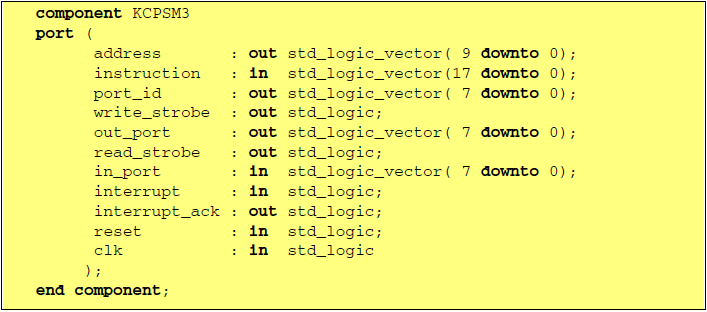
\includegraphics [width=300pt]{img/pico_declaration.png}
                            \caption{VHDL Component Declaration of KCPSM3}
                        \end{figure}
            %%%%%%%%%%%%%%%%%%%%%%%%%%%%%%%%%%%%%%%% instantiation
                                    \begin{figure}
                            \centering{}
                            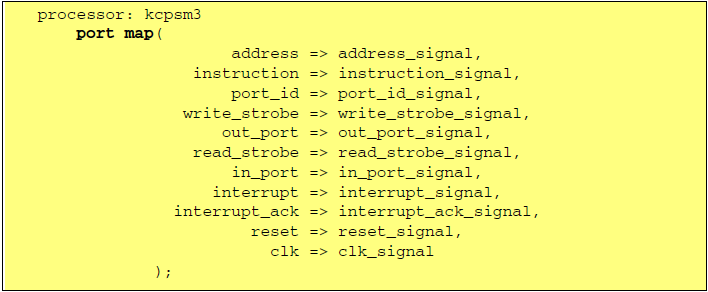
\includegraphics [width=300pt]{img/pico_instantiation.png}
                            \caption{VHDL Component Instantiation of the KCPSM3}
                        \end{figure}
            %%%%%%%%%%%%%%%%%%%%%%%%%%%%%%%%%%%%%%%%%%%%%%%%%%%%%%%%%%%%%%%%
                \subsection{Connecting the Program ROM}
                The PicoBlaze program ROM is used within a VHDL design flow. The PicoBlaze assembler
                generates a VHDL file in which a block RAM and its initial contents are defined. This
                VHDL file can be used for both logic synthesis and simulation of the processor.\\
                Next two figures shows the component declaration for the program ROM, and the component instantiation.
                The name of the program ROM, shown as "prog rom" in the
                following figures, is derived from the name of the PicoBlaze assembler source file. For
                example, if the assembler source file is named phone.psm, then the assembler generates a
                program ROM definition file called phone.vhd.
            %%%%%%%%%%%%%%%%%%%%%%%%%%%%%%%%%%%%%%%% declaration
                        \begin{figure}
                            \centering{}
                            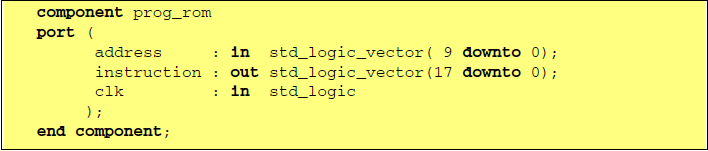
\includegraphics [width=300pt]{img/rom_declaration.png}
                            \caption{VHDL Component Declaration of Program ROM}
                        \end{figure}
            %%%%%%%%%%%%%%%%%%%%%%%%%%%%%%%%%%%%%%%% instantiation
                        \begin{figure}
                            \centering{}
                            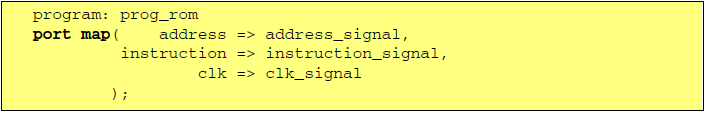
\includegraphics [width=300pt]{img/rom_instantiation.png}
                            \caption{VHDL Component Instantiation of Program ROM}
                        \end{figure}

\end{document} 

